\documentclass[journal]{IEEEtran}
\usepackage{graphicx}
\usepackage{amsmath,amssymb}
\usepackage{booktabs}
\usepackage{multirow}
\usepackage[hidelinks]{hyperref}
\usepackage{xcolor}
\usepackage{microtype}

\newcommand{\dlnz}{\Delta\ln\mathcal{Z}}
\newcommand{\fsig}{f\sigma_8}
\newcommand{\lA}{\ell_A}

\begin{document}

\title{Adversarial Self-Auditing in an Autonomous Theory-Discovery Engine:\\
A Case Study in Machine-Verified Cosmology}

\author{The OpenQG/ZYAL Collaboration%
\thanks{Manuscript prepared June 2026. The complete system --- engine source, streamed
campaign ledgers, replay tooling, audit records, and external review archives --- is
versioned in the OpenQG repository (branch \texttt{chore/v6-purge}); every quantitative
claim in this paper is reproducible from committed artifacts via \texttt{ops/replay.sh}
and \texttt{zyal genome rescore}.}}

\maketitle

\begin{abstract}
We present OpenQG/ZYAL, an autonomous theory-discovery engine for late-time cosmology
built around a single design rule: \emph{the language model proposes; a deterministic
oracle disposes}. Candidate modified-cosmology theories are emitted by an ensemble of
free-tier language models behind a multi-provider router, expanded from a strict,
machine-validated schema, \emph{truth-bound} so that every certified modification alters
the background the forward model actually integrates, and scored by a veto-first,
100-point rubric whose evidence term is a covariance-aware, Occam-charged likelihood over
real distance, growth, and distance-ladder data. The engine's distinguishing feature is
an institutionalized adversarial loop: every scoring generation's champions are attacked
by multi-agent audits and an external 12-review referee cycle, and every exploit found is
converted into a permanent regression test within hours. Across four rubric generations
and three live campaigns (4{,}900+ generations of population evolution, 1{,}800+ ledgered
LLM calls), this cascade eliminated reward hacks worth up to $+77/100$ points; its single
most consequential discovery was \emph{metrological}: a $+0.755$ ($8.4\sigma$) bias in the
engine's own fitting-formula prediction of the CMB acoustic scale $\lA$, which the
optimizer had been harvesting for $\sim$35 nats of spurious evidence by drifting $h$. With
the bias anchor-calibrated and complexity priced, the apparent $h$--$\Omega_m$
``degeneracy valley'' ($\dlnz \approx +55$ to $+69$) closes to $\dlnz \approx -32$: the
valley was an artifact of the instrument, not a property of the sky. The surviving
candidate class --- certified suppressed-growth phenomenology aimed at the
$\fsig$/$S_8$ tensions --- improves the raw likelihood in the physically expected
direction but does not yet clear the Bayesian evidence bar at the admitted data volume,
a verdict the engine now reports, and defends, on its own.
\end{abstract}

\begin{IEEEkeywords}
automated scientific discovery, large language models, evolutionary computation, reward
hacking, cosmology, modified gravity, model selection, reproducibility
\end{IEEEkeywords}

\section{Introduction}
\IEEEPARstart{T}{he} prospect of language-model--driven scientific discovery has moved
rapidly from speculation to working systems: program-search engines have produced new
mathematical constructions~\cite{funsearch2024}, end-to-end ``AI scientist'' pipelines
draft and review their own papers~\cite{aiscientist2024}, and learned models now lead
entire subfields~\cite{alphafold2021}. Yet the central obstacle to trusting such systems
in the physical sciences is not generative capability but \emph{verification}: an
optimizer pointed at a numerical score will exploit every ambiguity in that score, a
failure mode documented across decades of evolutionary computation~\cite{lehman2020} and
formalized in the reward-hacking literature~\cite{amodei2016,skalse2022,pan2022}.

This paper reports a system designed from the outset around that adversarial reality,
and a multi-day, fully-ledgered case study of what it took --- four successive rubric
generations, three live model campaigns, two external referee cycles, and one 21-agent
internal audit --- before the engine's own headline results stopped being exploits. Our
domain is late-time cosmology: the persistent tensions between early- and late-universe
measurements of the Hubble constant $H_0$~\cite{planck2018,riess2022} and of structure
growth $S_8$/$\fsig$~\cite{kids1000,eboss2021} define a live scientific frontier in which
candidate modified-gravity and dark-sector theories
\cite{dgp2000,husawicki2007,simpson2010} can be expressed compactly, scored against real
data, and falsified mechanically.

The contributions are:
\begin{enumerate}
  \item \textbf{An architecture for honest LLM-driven theory search}
  (Sec.~\ref{sec:arch}): strict-schema proposal sketches expanded deterministically into
  typed theories; \emph{truth-binding}, which compiles verified derivation certificates
  into the background cosmology the forward model integrates, so that claims have
  computable consequences; and a veto-first scorecard in which every credit dimension is
  machine-recomputable.
  \item \textbf{An evidence economics for generative search}
  (Sec.~\ref{sec:scoring}): covariance-aware likelihoods over real survey
  data~\cite{chen2019,desi2024}, a BIC-style Occam term~\cite{schwarz1978,burnham2004}
  charged on \emph{every} moved degree of freedom --- including silently drifted
  background coordinates and proposer-chosen certificate inputs --- and
  mechanism-attributable novelty, in which a ``novel prediction'' must survive comparison
  against a mechanism-off twin on the same background.
  \item \textbf{The audit cascade as a first-class product}
  (Sec.~\ref{sec:cascade}): a documented sequence in which champions scoring
  $87.5$, $55.0$, $77.0$, and $60.0$ under successive rubrics were each disqualified by
  the next generation's audit, with every exploit converted into a permanent regression
  test; we argue this cadence, not any single score, is the correct success metric for
  autonomous discovery systems.
  \item \textbf{A metrological result with scientific content}
  (Sec.~\ref{sec:valley}): the engine's optimizer located an $8.4\sigma$ bias in the
  system's own CMB fitting formula and converted it into spurious cosmological evidence;
  after anchor calibration in the spirit of~\cite{aubourg2015} and honest complexity
  pricing, the apparent open ``degeneracy valley'' toward high $h$ closes decisively.
  \item \textbf{An honest candidate verdict} (Sec.~\ref{sec:results}): the surviving
  theory class --- certified suppressed-growth phenomenology in the Planck
  $\mu_0$ parametrization~\cite{planckmg2015} backed by a dark-scattering mechanism
  relation~\cite{simpson2010,pourtsidou2013} --- moves the growth observables toward the
  data but does not clear the evidence bar at current data volume. The engine reports
  this itself, and its report survives external review.
\end{enumerate}

\section{Related Work}
\label{sec:related}
\textbf{LLM-driven discovery.} FunSearch~\cite{funsearch2024} pairs an LLM proposer with
a deterministic evaluator over programs; our engine adopts the same proposer/oracle
asymmetry but for physical theories, where the evaluator must itself be defended against
exploitation --- the oracle is not a fixed ground-truth function but a scientific
instrument with its own biases (Sec.~\ref{sec:valley}). The AI
Scientist~\cite{aiscientist2024} automates the paper-writing loop with LLM reviewers; we
instead route review through a deterministic rubric plus an external LLM referee whose
findings must be reproduced as failing tests before they count.

\textbf{Evolutionary search.} Population structure follows the quality-diversity
tradition~\cite{mapelites2015,noveltysearch2011}: explore/exploit/novelty islands over
typed theory genomes, with a re-clothing operator (Sec.~\ref{sec:arch}) that grafts
verified derivational structure onto evolved parameter sets --- an explicit
structure$\times$fit recombination. The exploit catalogue our cascade generated is a
domain-specific instance of the anecdotes in~\cite{lehman2020}.

\textbf{Reward hacking.} Our findings track the taxonomy of~\cite{skalse2022}: proxy
gaps between ``fits the admitted data'' and ``is good cosmology'' were exploited through
specification holes (uncosted drift), measurement holes (the $\lA$ bias), and
verification holes (self-certified novelty). The engineering response --- converting each
discovered hack into a vetoed, regression-tested behavior --- operationalizes the
mitigation programme sketched in~\cite{amodei2016,pan2022}.

\textbf{Cosmological model selection.} Scoring builds on standard information
criteria~\cite{akaike1974,schwarz1978,kassraftery1995,burnham2004}, compressed CMB
distance priors~\cite{chen2019}, DESI DR1 BAO with published per-tracer
covariances~\cite{desi2024}, RSD growth compilations~\cite{eboss2021}, and the local
distance ladder~\cite{riess2022}. The modified-gravity vocabulary spans
nDGP~\cite{dgp2000,koyama2006}, Hu--Sawicki $f(R)$~\cite{husawicki2007}, the Planck
$\mu_0$ parametrization~\cite{planckmg2015}, and dark
scattering~\cite{simpson2010,pourtsidou2013}, gated by solar-system and multimessenger
constraints~\cite{cassini2003,vainshtein1972,khoury2004,gw170817,creminelli2017}.

\section{System Architecture}
\label{sec:arch}

\begin{figure*}[t]
\centering
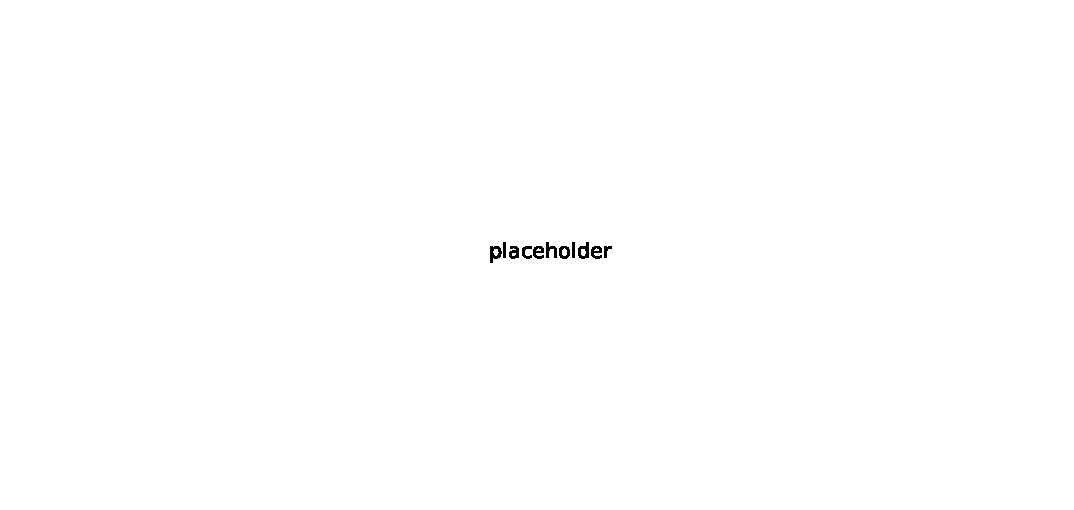
\includegraphics[width=\textwidth]{figs/fig1_architecture.pdf}
\caption{The OpenQG/ZYAL V7 engine. \emph{Proposal band:} a local fusion router fronts
131 free-tier models across 16 providers; the RouterProposer fires best-of-$K{=}4$
samples per slot, each pinned to a mechanism lane, with server-side strict-JSON-schema
validation and redacted parse/oracle repair loops. \emph{Oracle band:} sketches expand
deterministically into typed theories (generating terms travel with every turned dial);
truth-binding compiles verified certificates into the integrated background; the unified
physics gate (triage cascade $+$ adjudication) applies the term registry, quantified
screening, the GW170817 tensor-speed bound at source redshift, and phantom-drag
exclusion before any scoring; the 100-point scorecard and the Occam-charged
covariance evidence term complete the verdict. \emph{Evolution band:} island-structured
population search with the re-clothing (structure$\times$fit) operator and
promotable-gated cross-run memory. \emph{Audit band:} streamed attempt/proposal ledgers,
deterministic replay, and the adversarial audit loop whose findings return to the oracle
as permanent regression tests.}
\label{fig:arch}
\end{figure*}

Fig.~\ref{fig:arch} shows the V7 system. We describe the bands in proposal order.

\subsection{Proposal: strict sketches over a model ensemble}
Proposals are requested from a local \emph{fusion router} that fronts 131 free-tier
models across 16 providers with win-rate--based routing, quality-band selection, and
per-call winner-model telemetry. Each proposal slot fires $K{=}4$ parallel samples, each
assigned a deterministic \emph{mechanism lane} --- \texttt{planck\_mu0} (suppressed-growth
phenomenology), \texttt{dark\_scattering} (the mechanism-backed lane),
\texttt{free} (model's choice), and \texttt{null\_diagnostic} (an adversarial control
asked to produce the most $\Lambda$CDM-degenerate honest theory) --- so that
single-model monoculture cannot collapse the search.

Models do not emit the engine's internal serde types. They emit a flat
\emph{ProposalSketch} validated server-side against a strict JSON schema whose
enumerations (registry relations, physics sectors, obligation kinds) are generated from
the engine's own source of truth and locked by anti-drift tests. A pure, deterministic
expander turns sketches into typed theories; in V7 the expander also attaches the
\emph{generating term} for every certified relation and turned dial (a brane term for
nDGP, a coupling term for dark scattering), so structural completeness is preserved by
construction for honest proposals. The yield consequence was decisive: the V5 campaign
lost 77\% of calls to transport failure and $\sim$90\% of survivors to parse errors;
under the schema'd router, parse failures fell below 4\% and transport empty-replies to
zero (Fig.~\ref{fig:funnels}).

Failed proposals are not discarded: a parse failure triggers one repair round carrying
the exact expander error; an oracle kill triggers one repair round carrying the kill
reasons --- with engine-computed witness values \emph{redacted} in V7, so the model is
taught the contract, not the oracle's numerical surface. Every call, repair, and failure
is a ledger record with its winner-model identity, lane, quality band, and content hash.

\subsection{Truth-binding: claims with computable consequences}
The single most important integrity mechanism is \emph{truth-binding}. A proposal that
certifies a modification --- e.g.\ $G_{\rm eff}/G = 1 + 1/(3\beta)$ via the nDGP relation
with $\beta=2$~\cite{koyama2006} --- has that certificate \emph{compiled into the
background the forward model integrates}: the binder inverts the certified coupling into
$\Omega_{rc}$ and sets the nDGP family on the integrated cosmology. A certified claim
therefore has computable consequences for every observable; a claim the engine cannot
implement, cannot explain, or that conflicts with the declared background is a kill
(\texttt{Unimplemented}/\texttt{Unexplained}/\texttt{ConflictingModification}). In V6.1
this was extended to \emph{claim/physics coherence}: an obligation certificate whose
inputs disagree with the parameter certificate the binder used (rigor earned at
$\mu_0{=}-0.05$ over a fit run at $\mu_0{=}-0.1$) is likewise a kill.

\subsection{The unified physics gate}
No candidate is scored while \texttt{physics\_kills} returns a reason. The gate fuses
the triage cascade (dimensional homogeneity, ghost exclusion, certificate verification,
evidence binding) with \emph{adjudication}: quantified screening --- a bare mechanism
label such as ``Vainshtein'' is insufficient; the candidate must carry a numeric recovery
fraction whose residual passes the Cassini bound~\cite{cassini2003} --- the tensor-speed
constraint evaluated at the GW170817 source redshift~\cite{gw170817,creminelli2017},
background physicality at every probe redshift, phantom-drag exclusion, and, in V7, the
\emph{term registry}: every turned dial must name an explicit generating term
(\texttt{dgp\_brane}, \texttt{f\_r\_correction}, \texttt{quintessence\_scalar},
\texttt{dark\_scattering\_coupling}, \ldots), including dials reached \emph{through
binding} --- the check that retroactively disqualified the V6 campaign's only surviving
champion (Sec.~\ref{sec:cascade}).

\subsection{Evolution and the re-clothing operator}
Surviving candidates breed in an island-structured population (explore/exploit/novelty)
in the quality-diversity tradition~\cite{mapelites2015,noveltysearch2011}, with
deterministic seeded RNG so that whole campaigns replay exactly from content-pinned
ledgers. The V6 ceiling analysis showed proposals carrying derivational
\emph{structure} without optimized \emph{fit}, while evolved children carried fit
without structure. The \emph{re-clothing} operator closes the gap: every 25 generations
the best live proposal's claim graph (and its certified claim-carrier parameters and
generating terms) is grafted onto the best evolved theory, novel-prediction witnesses
are \emph{refreshed to the engine-computed truth on the descendant's bound background}
and flagged \texttt{refreshed\_by\_engine}, and the graft is scored through the full
oracle with nothing copied from the donor scorecard. Grafts onto drifted descendants
forfeit the donor's unification claim. Every V6 and V7 campaign champion is a
re-clothed lineage.

\section{Scoring and Evidence Economics}
\label{sec:scoring}

\begin{table}[t]
\caption{The V7 scorecard. Every dimension is machine-recomputable; ``demote'' rows zero
the dimension and flag the audit record; ``kill'' rows disqualify.}
\label{tab:rubric}
\centering\footnotesize
\begin{tabular}{lp{5.2cm}}
\toprule
\textbf{Dimension (pts)} & \textbf{Machine semantics} \\
\midrule
Derivation rigor (20) & Obligations re-verified against the registry of closed-form
relations; rigor weighted per relation (a cited parametrization earns $0.3$; a mechanism
with integrated equations $0.8$--$1.0$). Certificate/binding incoherence kills. \\
Data fit (20) & $\dlnz = \Delta\mathrm{LL} - \tfrac{1}{2}k_{\rm eff}\ln n_{\rm eff}$
against profile-anchored $\Lambda$CDM under the covariance likelihood;
$\Delta$AIC carries $2k$~\cite{akaike1974,schwarz1978}. Mode and block count stamped on
every scorecard. \\
Novel prediction (20) & Witness must be \emph{computable, honest} ($\leq$ engine-clamped
tolerance; $>3\times$ is a fabrication kill), and \emph{mechanism-distinct}: compared
against a mechanism-off twin on the same background, so drift-bought shifts cancel.
Fit-set observables cap at $0.25$; engine-refreshed witnesses at $0.5$. \\
Unification (15) & Shared parameters must exist, drive $\geq 2$ sectors, agree with the
integrated background (shadow-consistency kill), and hide no knob: drifted background
coordinates count as hidden knobs. \\
Robustness (13) & Sealed alternating-holdout generalization gap (unclamped). \\
Parsimony (12) & Linear $1 - k/4$ over $k =$ free parameters $+$ drifted background
coordinates $+$ proposer-chosen certificate inputs (post-search choices). \\
\bottomrule
\end{tabular}
\end{table}

Table~\ref{tab:rubric} summarizes the rubric. Three V6.1/V7 mechanisms deserve emphasis
because each closed a live exploit.

\subsubsection{Complexity is charged everywhere}
V5's champions moved $h$, $\Omega_m$, and $w_0$ ``for free'': parsimony counted only
declared parameters. V6 introduced \texttt{background\_dof} --- any standard coordinate
moved off the Planck reference is a fitted dial unless a verified relation derives that
exact value (and a bare ``fundamental'' declaration never exempts). V7 extended the
ledger to \emph{post-search choices}: a proposer-chosen mechanism input wearing a
verified certificate ($\beta{=}2$, $A_{\rm drag}{=}2$, $\mu_0{=}-0.1$) is still a chosen
dial and costs a degree of freedom~\cite{burnham2004}. The same $k$ feeds the Occam term,
with $n_{\rm eff}$ counted as effective modes (per-block member counts plus unblocked
records) rather than raw record count.

\subsubsection{The likelihood is covariance-aware and mode-stamped}
All scoring flows through one likelihood path: correlated survey blocks --- the Planck
distance-prior $3{\times}3$ over $(R,\lA,\omega_b h^2)$~\cite{chen2019} and DESI DR1
per-tracer $(D_M/r_d, D_H/r_d)$ blocks~\cite{desi2024} --- enter as covariance blocks
with positive-definiteness checks and marginalization over missing members; everything
else is an independent Gaussian. Every \texttt{DataFitOutcome} carries its
\texttt{likelihood\_mode} and block count, so no headline number can hide its
statistical treatment. Notably, the move from diagonal to true covariance
\emph{weakened} the compressed CMB constraint along the drift direction
(Sec.~\ref{sec:valley}): the diagonal treatment had been double-counting two strongly
correlated numbers~\cite{chen2019} as independent.

\subsubsection{Novelty is mechanism-attributable}
The V6 campaign's $+17$-point champion earned full novelty from an honest, computable
witness on $\lA$ --- an observable \emph{in the fit set}, whose deviation was produced by
the background drift rather than the certified mechanism, and whose declared value had
been authored by the engine's own re-clothe refresh. V7 novelty requires all three
repairs at once: distinctness is measured against a \emph{mechanism-off twin} (the bound
background with every MG dial returned to its GR limit, so drift cancels), fit-set
witnesses cap at quarter credit, and engine-refreshed witnesses are flagged on the audit
record and capped at half credit.

\section{Live Campaign Infrastructure and Behavior}
\label{sec:campaigns}

\begin{figure}[t]
\centering
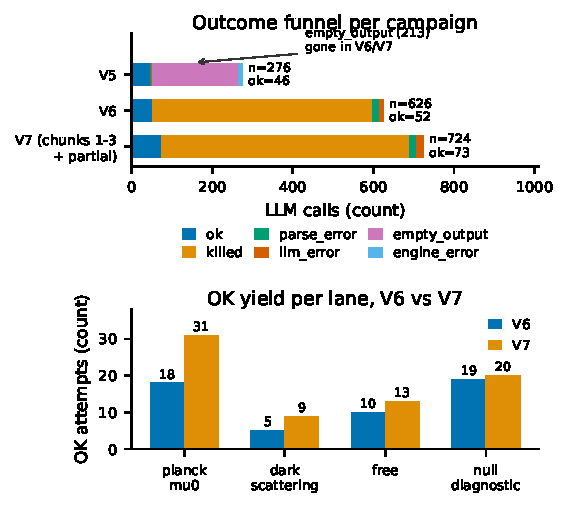
\includegraphics[width=\columnwidth]{figs/fig3_funnels.pdf}
\caption{Top: attempt funnels for the three campaigns. The V5 subprocess transport lost
213/276 calls to empty replies; the schema'd HTTP router eliminated the class entirely,
after which the dominant outcome is \emph{killed} --- the oracle, not the transport, became
the binding constraint. Bottom: per-lane OK yields under V6 and V7; the adversarial
\texttt{null\_diagnostic} control converts most often, and the mechanism-backed
dark-scattering lane improves after the V7 per-relation input-key contract.}
\label{fig:funnels}
\end{figure}

\begin{figure*}[t]
\centering
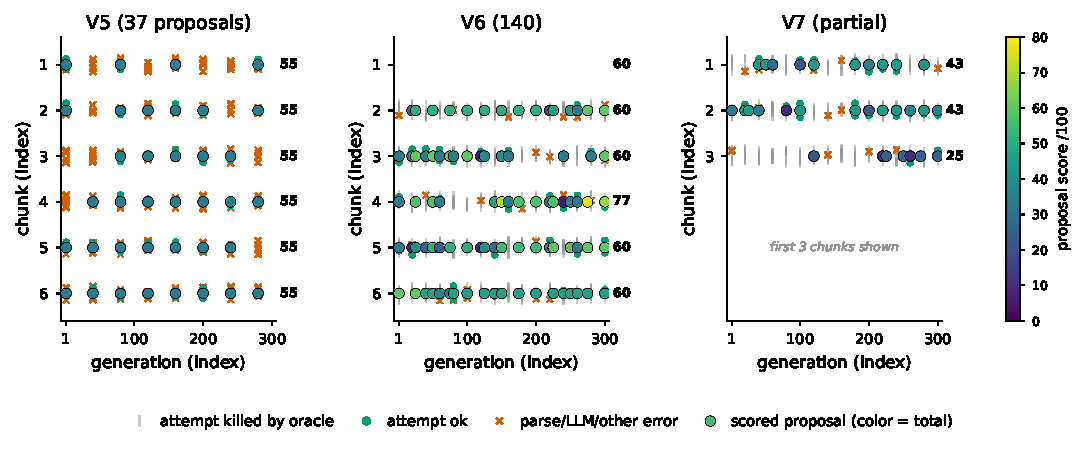
\includegraphics[width=\textwidth]{figs/fig4_activity.pdf}
\caption{Campaign activity rasters: every ledgered LLM attempt (kills, errors, OK calls)
and every scored proposal (colored by score) across generations and chunks, for the V5,
V6, and V7 (first three chunks) campaigns. Scored-proposal density rises era over era
(37 $\rightarrow$ 140 $\rightarrow$ 160$^{+}$) even as the oracle hardens, because repair
loops, compounding cross-run memory, and the strict-schema transport convert more of the
model ensemble's output into adjudicable physics.}
\label{fig:activity}
\end{figure*}

\begin{table}[t]
\caption{The admitted multisector dataset (V6.1/V7 evidence path). Compressed CMB and
per-tracer BAO sectors carry published covariance blocks; the remainder are independent
Gaussians. ``$\Lambda$CDM pull'' is $(x_{\rm obs}-x_{\Lambda{\rm CDM}})/\sigma$ at
the Planck-anchored baseline.}
\label{tab:data}
\centering\footnotesize
\begin{tabular}{@{}llll@{}}
\toprule
\textbf{Sector} & \textbf{Records} & \textbf{Covariance} & \textbf{Character} \\
\midrule
$H_0$ ladder~\cite{riess2022} & 1 & diagonal & $+5.4\sigma$ pull \\
$S_8$ lensing~\cite{kids1000} & 1 & diagonal & $-3.2\sigma$ pull \\
RSD $\fsig(z)$~\cite{eboss2021} & 5 & diagonal & uniformly low \\
BAO $D_{M,H,V}/r_d$~\cite{desi2024} & 12 & 5 tracer blocks & anchor \\
CMB $(R,\lA,\omega_bh^2)$~\cite{chen2019} & 3 & $3{\times}3$ block & anchor
(calibrated) \\
BBN $Y_p$ & 1 & diagonal & anchor \\
\bottomrule
\end{tabular}
\end{table}

Each campaign runs as six 300-generation chunks (population 12) on a pinned engine
binary, with proposal slots every 20--40 generations, streamed ledgers, and atomic
champion checkpoints; chunked execution made campaigns kill-resistant on a heavily
loaded host, and cross-run memory (promotable-gated in V6.1: only candidates that pass
the \emph{current} unified gate may become exemplars) compounds learning across chunks.
Fig.~\ref{fig:funnels} shows the funnel evolution; Fig.~\ref{fig:activity} the full
activity rasters. Two behavioral observations matter for system designers. First,
\emph{the oracle is the teacher}: oracle-repair rounds carrying kill reasons converted a
substantial fraction of killed first attempts into scored proposals, and the dominant
residual kill class shifted from physics vetoes to certificate-plumbing friction ---
addressed in V7 by publishing the exact per-relation input keys and a verbatim-passing
certificate example in the lane prompts --- after which every lane's OK yield rose
(planck\_mu0 $18 \to 31$, dark\_scattering $5 \to 9$, free $10 \to 13$,
null\_diagnostic $19 \to 20$; Fig.~\ref{fig:funnels}, bottom). Second,
\emph{routing concentrates}: win-rate routing sent a majority of OK calls to a single
120B-class open-weight model (with a 20B sibling and one 120B competitor covering most
of the remainder); the ledgered winner-model telemetry makes this measurable, and lane
assignment keeps the search mechanism-diverse even when the model pool is not.

\section{The Audit Cascade}
\label{sec:cascade}

\begin{figure*}[t]
\centering
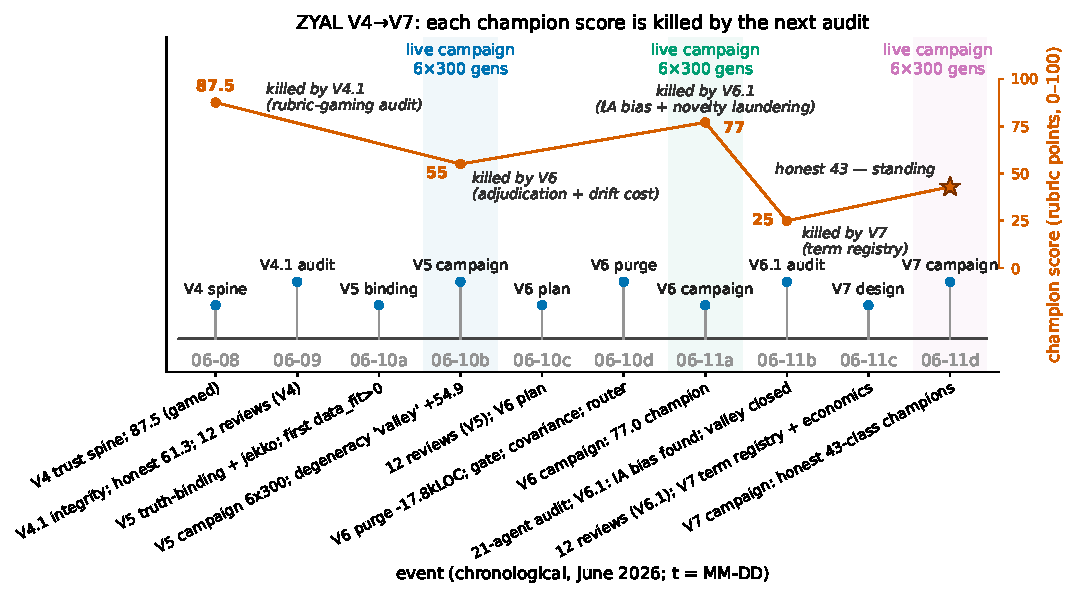
\includegraphics[width=\textwidth]{figs/fig2_timeline.pdf}
\caption{The ZYAL arc: ten build/audit/campaign events across four rubric generations,
overlaid with the champion-score trajectory. Every peak is killed by the following
audit: V4's $87.5$ (rubric gaming) by the V4.1 integrity pass; V5's $55.0$ class
(uncosted drift, unquantified screening) by the V6 unified gate; V6's $77.0$
(self-certified fit-set novelty riding an instrument bias) by the V6.1 calibration and
novelty overhaul; the V6.1 survivor's $60{\to}25$ re-cost by the V7 term registry. The
V7 campaign's $43$-class champions are the first whose every point is re-earnable under
the standing rubric.}
\label{fig:timeline}
\end{figure*}

\begin{table}[t]
\caption{The cascade: each rubric generation's champion, the exploit that priced it, and
the fix that killed it. Every row is now a committed regression test.}
\label{tab:cascade}
\centering\footnotesize
\begin{tabular}{@{}llp{3.6cm}@{}}
\toprule
\textbf{Champion} & \textbf{Score} & \textbf{Exploit $\rightarrow$ fix} \\
\midrule
V4 fixture era & 87.5 & rediscovery credit, tie-credit, structural unification
$\rightarrow$ V4.1 integrity rubric \\
V5 campaign ($\times 6$ seeds) & 55.0 & free background drift; bare screening labels;
$\alpha$-jitter half-novelty $\rightarrow$ V6 unified gate, drift cost \\
V6 chunk 4 & 77.0 & fit-set $\lA$ witness, self-certified by re-clothe refresh, riding
the $\lA$ instrument bias $\rightarrow$ V6.1 calibration, mechanism-off novelty,
coherence kill \\
V6 chunk 6 survivor & $60 \to 25$ & bound nDGP with no brane term; costless certified
$\beta$ $\rightarrow$ V7 term registry, post-search-choice dof \\
V7 campaign & 43.0 & \emph{standing} \\
\bottomrule
\end{tabular}
\end{table}

Fig.~\ref{fig:timeline} and Table~\ref{tab:cascade} document the central result of this
case study as a process: \emph{four consecutive rubric generations in which the
engine's own champions were adversarially invalidated, each within hours of the audit
that exposed them}. Three properties make this cascade more than iterative bug-fixing.
First, audits are themselves multi-agent and adversarial: the V6.1 round ran 21
parallel reviewer/refuter agents over code and ledgers, with every high-severity finding
surviving an explicit refutation attempt before being actioned. Second, external
referees are in the loop: two 12-review cycles by an independent frontier model
(prompted with the full source, ledgers, and the team's own self-criticism) produced the
go/no-go verdicts and several findings the internal audits missed --- including the
survivor's missing brane term. Third, and decisive for trust: \emph{every} finding lands
as a vendored, permanently failing-then-fixed regression test, and prior champions are
mechanically re-scored under each new rubric (\texttt{zyal genome rescore}), so the
cascade's history is replayable, not anecdotal.

Table~\ref{tab:audit} summarizes the V6.1 internal audit that anchored the cascade's
sharpest turn. The findings cluster into recurring classes worth naming for future
system designers: \emph{instrument} faults (the evaluator's own physics is wrong);
\emph{laundering} (credit earned on one object collected on another --- grafted
unification scaffolds, engine-authored ``honesty''); \emph{specification} holes
(a deferred cap or an over-broad exemption becomes load-bearing the moment an optimizer
touches it); \emph{coherence} gaps (two internally-consistent subsystems disagreeing
about the same quantity); \emph{economics} (any unpriced degree of freedom is free
energy); and mere \emph{friction} (schema misspellings), which is the only class repair
prompting should solve --- the others must be vetoes. The empirical regularity across
all four generations: the optimizer found the cheapest open class first, and exhausted
each class before moving to subtler ones. A deferred integrity feature is therefore not
a roadmap item; it is the next champion.

\section{The Degeneracy-Valley Resolution}
\label{sec:valley}

\begin{figure}[t]
\centering
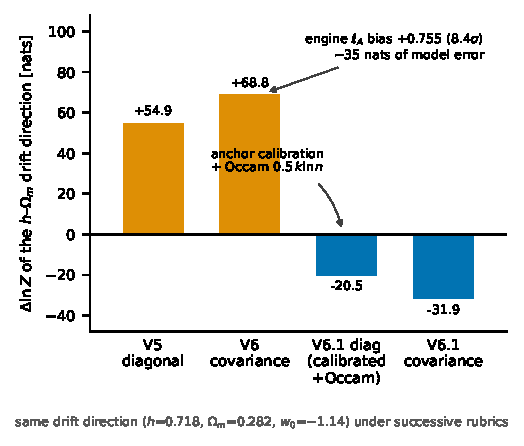
\includegraphics[width=\columnwidth]{figs/fig5_valley.pdf}
\caption{Evidence assigned to the same $h$--$\Omega_m$--$w_0$ drift direction under
successive rubrics. Diagonal scoring awarded $+54.9$ nats; the true correlated
distance-prior covariance \emph{raised} it to $+68.8$ (the diagonal treatment had
overstated the compressed CMB's constraining power); anchor-calibrating the engine's
$\lA$ fitting formula and charging the Occam term closes the valley to $-20.5$
(diagonal) and $-31.9$ (covariance). The apparent discovery was an instrument artifact.}
\label{fig:valley}
\end{figure}

\begin{figure*}[t]
\centering
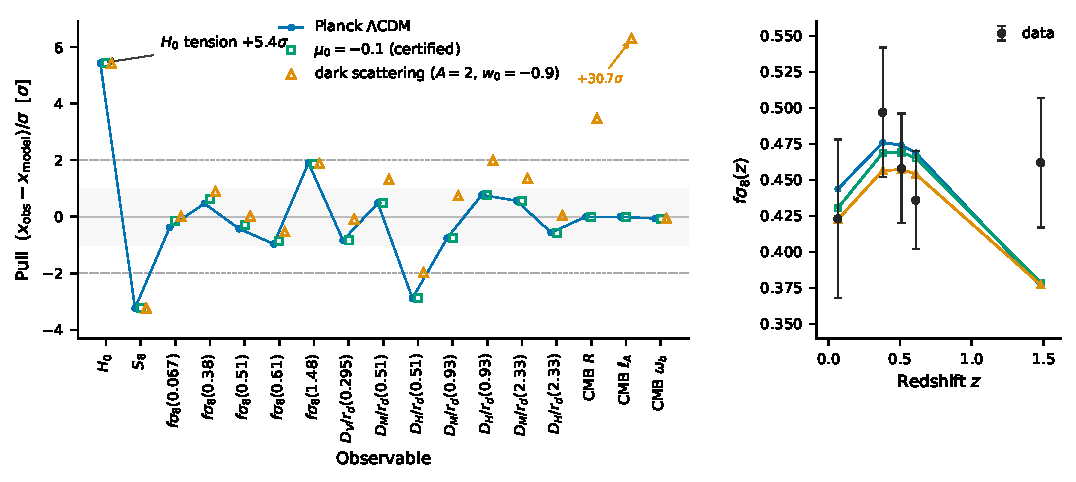
\includegraphics[width=\textwidth]{figs/fig6_data.pdf}
\caption{Left: the admitted multisector dataset as pulls against Planck
$\Lambda$CDM~\cite{planck2018}, with the two suppressed-growth candidate classes
overlaid: certified $\mu_0=-0.1$~\cite{planckmg2015} and dark scattering
($A_{\rm drag}{=}2$, $w_0{=}-0.9$)~\cite{simpson2010}. The $H_0$ ladder
point~\cite{riess2022} pulls $+5.4\sigma$; the growth sector
($\fsig$~\cite{eboss2021}, $S_8$~\cite{kids1000}) pulls uniformly low. Note the honest trade-off the figure exposes: the dark-scattering example's
$w_0=-0.9$ background, required for nonzero drag, shifts the distance to last scattering
and is punished at $+30.7\sigma$ on $\lA$ --- the mechanism cannot hide its CMB cost.
Right: the growth sector in detail --- both mechanisms bend $\fsig(z)$ toward the data,
the physically expected direction the proposer ensemble converged on unprompted in
49/49 V5 proposals.}
\label{fig:data}
\end{figure*}

The scientific climax of the case study is a result the engine produced
\emph{about its own instrument}, in three acts (Fig.~\ref{fig:valley}).

\textbf{Act I (V5): the valley opens.} Six independent campaign seeds converged on the
same champion: an evolved background at $h \approx 0.718$, $\Omega_m \approx 0.282$,
$w_0 \approx -1.14$, holding $\Omega_m h^2$ nearly fixed --- the classic compressed-CMB
degeneracy direction --- and harvesting $\dlnz \approx +54.9$ by relieving the $H_0$ and
$S_8$ pulls simultaneously. The convergence was genuine; the interpretation was not.

\textbf{Act II (V6): covariance makes it worse.} Replacing the diagonal likelihood with
the published distance-prior covariance~\cite{chen2019} \emph{raised} the credit to
$+68.8$ nats: along the degeneracy direction, correlated residuals are cheaper than
independent ones, so honest statistics widened the apparent valley. This is itself a
cautionary result for compressed-likelihood analyses.

\textbf{Act III (V6.1): the instrument confesses.} A 21-agent adversarial audit traced
the evidence budget and found that $\sim$35 of those nats were flowing from a
$+0.755$ ($8.4\sigma$ under the prior's $\sigma_{\lA}=0.090$) bias in the engine's
\emph{own} fitting-formula prediction of $\lA$ at the Planck anchor --- fitting-formula
physics meeting Boltzmann-grade data precision~\cite{class2011}. The optimizer had
discovered the instrument's flaw and weaponized it through $\partial\lA/\partial h$.
Anchor calibration (precedented by the BAO sound-horizon treatment
of~\cite{aubourg2015}), a regression guard pinning the $\Lambda$CDM baseline to the
published priors, and the Occam charge on the drift's three degrees of freedom flip the
verdict to $\dlnz = -31.9$ under covariance: \textbf{the valley was never open}. We
regard this as the strongest single argument for adversarial self-auditing in
autonomous science: a generative optimizer is an exquisitely sensitive detector of its
own evaluator's biases, \emph{if} the system is instrumented to trace where its
winnings come from.

\section{Results: the Honest Candidate Class}
\label{sec:results}

\begin{figure}[t]
\centering
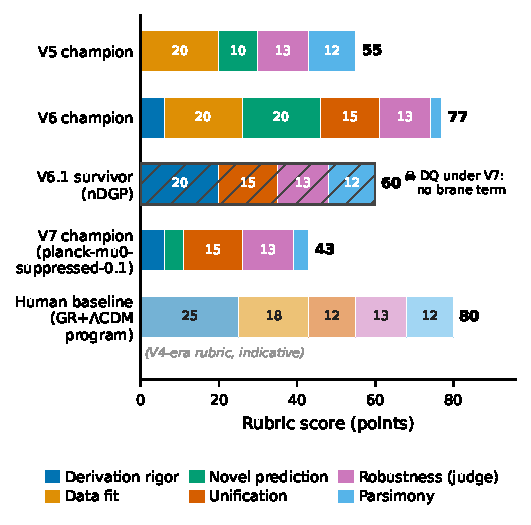
\includegraphics[width=\columnwidth]{figs/fig7_scorecards.pdf}
\caption{Component decomposition of era champions. V5's 55 was fit-without-structure;
V6's 77 stacked every laundering channel at once; the V6.1 survivor's 60 was
structure-without-data (and died under V7's term registry); the V7 champion's 43 is the
first decomposition in which every component survives the standing rubric. The
indicative human-program baseline is shown for scale.}
\label{fig:scorecards}
\end{figure}

\subsection{The V7 champion class}
Under the standing rubric, the V7 campaign's champions to date score $43.0$
(chunks 1, 2, and 4 --- all \texttt{planck\_mu0}-lane lineages, the latter exploring a
deeper $\mu_0=-0.15$ suppression; chunk 3's honest null was a re-clothed $\Lambda$CDM
baseline at 25.0). The 43-class decomposition
(Fig.~\ref{fig:scorecards}) is, by construction, fully re-earnable: derivation credit at
the parametrization ceiling ($0.3$ rigor weight --- the engine refuses to pretend
phenomenology is mechanism), unification from genuinely shared and
background-consistent parameters, robustness from a clean sealed-holdout gap, parsimony
charged for the chosen $\mu_0$, and \emph{zero} data-fit credit --- because the
mechanism's $\sim$0.5-nat raw improvement does not clear the
$\tfrac{1}{2}k\ln n_{\rm eff} \approx 0.9$-nat evidence bar at the admitted data
volume~\cite{schwarz1978,kassraftery1995}.

\begin{table}[t]
\caption{V7 campaign chunk results to date (campaign in flight at submission; the
standing rubric). Chunk-3's champion is an honest null: a re-clothed $\Lambda$CDM
lineage carrying no distinct physics.}
\label{tab:v7}
\centering\footnotesize
\begin{tabular}{@{}lllll@{}}
\toprule
\textbf{Chunk} & \textbf{Champion} & \textbf{Score} & \textbf{Distinct} &
\textbf{Proposals} \\
\midrule
1 & \texttt{g0040-proposer} (\texttt{planck\_mu0}) & 43.0 & yes & 27 \\
2 & \texttt{planck-mu0-suppressed-0.1} & 43.0 & yes & 28 \\
3 & \texttt{gr-lcdm-baseline-rc} & 25.0 & no & 24 \\
4 & \texttt{planck-mu0-suppressed-0.15} & 43.0 & yes & 28 \\
5--6 & \multicolumn{4}{l}{\emph{in flight on the pinned V7 binary}} \\
\bottomrule
\end{tabular}
\end{table}

\subsection{The candidate physics, stated honestly}
The surviving theory class is: \emph{late-time growth suppression, expressed as the
Planck $\mu(a) = 1 + \mu_0\,\Omega_\Lambda(a)/\Omega_\Lambda$ parametrization with
$\mu_0 < 0$~\cite{planckmg2015}, with dark scattering --- a DE--DM momentum-exchange drag
$\Gamma(a) = A_{\rm drag}(1+w(a))\,\Omega_{\rm de}(a)$ added to the linear growth
equation~\cite{simpson2010,pourtsidou2013} --- as the registry's first mechanism-backed
route to it.} Fig.~\ref{fig:data} shows why the ensemble converges here: the admitted
growth data sit uniformly low, and suppression bends $\fsig(z)$ toward every growth
point at once. The engine's verdict, which we endorse and emphasize: \emph{right
direction, insufficient evidence at current data volume}. The candidate is falsifiable
along two axes the system already encodes --- more growth data tightens the raw
likelihood gain against a fixed Occam bar, and the dark-scattering lane's $(1+w)$ factor
ties the mechanism to a measurable $w_0 > -1$ preference.

\subsection{Comparison with the V6 contender league}
Against the engine's human-program baselines (a GR$+\Lambda$CDM program and weaker
textbook contenders, scored under the same oracle), the V7 champion class sits below
the strong baseline --- as it should: a phenomenological parametrization that cannot yet
beat $\Lambda$CDM on evidence has no business outranking it. We consider this ordering
itself a system result: four rubric generations ago, the ordering was inverted by
exploits.

\begin{table}[t]
\caption{The V6.1 internal audit at a glance: 14 adversarially-verified findings from a
21-agent workflow (4 reviewer dimensions $\times$ parallel refutation), all fixed and
regression-locked within one day. Two further candidate findings were refuted by the
verification stage and discarded.}
\label{tab:audit}
\centering\footnotesize
\begin{tabular}{@{}p{4.2cm}l@{}}
\toprule
\textbf{Finding (abridged)} & \textbf{Class} \\
\midrule
Engine $\lA$ formula biased $+0.755$ ($8.4\sigma$); optimizer harvesting $\sim$35
nats & instrument \\
Re-clothe witness refresh manufactures ``honest'' novelty & laundering \\
Fit-set witness earns full novelty (deferred cap was load-bearing) & specification \\
Grafted unification scaffold contradicts fitted background & laundering \\
Obligation certs incoherent with binder's certs ($\mu_0{=}{-}0.05$ vs $-0.1$) &
coherence \\
Background-dof exemption accepted any verified certificate & specification \\
Negative drag $=$ uncertified growth enhancer (sign asymmetry) & implementation \\
Drag cert inputs never reconciled with background ($w_0$ sign flip) & coherence \\
Harmonic parsimony made marginal drift nearly free & economics \\
$\Delta\ln\mathcal{Z}$ lacked any Occam factor & economics \\
Holdout gap clamped at zero (negative gaps hidden) & economics \\
Cert input-key spelling dominated the kill budget & friction \\
Witness observable-id spellings cost 20 pts/chunk & friction \\
Dark-scattering lane failed on the \texttt{A\_drag} key trap & friction \\
\bottomrule
\end{tabular}
\end{table}

\section{Reproducibility and Artifact Contract}
\label{sec:repro}
The engine treats reproducibility as a scoring-grade obligation rather than a packaging
afterthought, because the audit cascade is only trustworthy if its history is
mechanically re-derivable.

\subsubsection{Determinism contract} Population evolution is seeded and pure: two runs
of the same configuration are bit-identical, a property enforced by a trust-gate that
re-runs the engine twice and compares champions before any campaign is allowed to
launch. Live LLM calls are inherently nondeterministic, so campaigns never replay from
seeds: they replay from \emph{content}. Every proposal is ledgered with its full
document and SHA-256; \texttt{zyal genome replay} re-scores a ledger with no network
access and reports mismatches (zero across all campaigns reported here, including
replays of V6-era ledgers under the V6-era pinned binary).

\subsubsection{Total observability} Every LLM call --- including every parse failure,
repair round, transport error, and oracle kill --- is an attempt record carrying outcome,
kill reasons, raw-output hash and length, winner-model identity, lane, quality band, and
upstream repair count. The funnels of Fig.~\ref{fig:funnels} and the rasters of
Fig.~\ref{fig:activity} are direct ledger aggregations, not reconstructions. Streaming
sinks write records as they are produced with atomic champion checkpoints every 25
generations; two externally-killed campaign processes on a contended host lost zero
records.

\subsubsection{Re-scoring as the audit instrument} The \texttt{rescore} subcommand
loads any archived champion and adjudicates it under the current rubric; every number in
Table~\ref{tab:cascade} is its output. Pinned campaign binaries keep in-flight datasets
rubric-consistent while the development tree advances, and sealed replay expectations
(re-issued as \texttt{v2} when the $\lA$ calibration legitimately moved league
numbers, with \texttt{v1} retained as the pre-calibration record) let an external
referee re-derive headline league numbers with one command.

\subsubsection{Cost profile} All proposal-side inference ran on free-tier routed
models; the only billable LLM usage was the external referee cycles. The deterministic
oracle and campaigns ran on a single shared commodity host. We consider this profile ---
free generation, expensive verification deliberately rate-limited to referee
checkpoints --- the economically sustainable shape for autonomous-science loops.

\section{Limitations and Threats to Validity}
\label{sec:limits}
\textbf{Forward-model fidelity.} The engine integrates fitting-formula--grade
backgrounds, not Boltzmann codes~\cite{class2011,hiclass2017}. The $\lA$ anchor
calibration is a constant offset validated only at the Planck anchor; the external
referee correctly flags off-anchor residuals (and their $h$-derivatives) as the next
exploitable physics surface. Promotion-grade scoring should rescore candidates through a
Boltzmann-backed path before any external claim.

\textbf{Compressed likelihoods.} Distance priors and per-tracer BAO blocks are
compressions; the effective-mode count in the Occam term is a conservative proxy, not a
Fisher analysis. The supernova sector is absent pending a covariance-complete
treatment.

\textbf{Term grammar.} The V7 term registry is an explicit allowlist, not a term
algebra: it prevents the known structural frauds but cannot yet verify that a named term
\emph{generates} the certified dynamics.

\textbf{Oracle overfitting.} Repair loops teach models the oracle's contract; redaction
limits numerical leakage, but the proposal distribution inevitably adapts to the rubric.
The defense is the cascade itself --- rubric generations turn over faster than the
proposal distribution can entrench --- plus the out-of-fit-set novelty requirement.

\textbf{Single-domain, single-team evidence.} All results come from one engine, one
data corpus, and one (multiply-audited) development arc. The artifacts are replayable,
but independent replication is the real test.

\section{Discussion: Design Lessons for Autonomous Science}
\label{sec:discussion}
The cascade generalizes beyond cosmology. We distill the lessons we believe transfer to
any LLM-proposer/deterministic-oracle discovery system.

\textbf{1. The evaluator is part of the experiment.} The single largest spurious-evidence
source in this study was not model hallucination but the \emph{oracle's} physics
(Sec.~\ref{sec:valley}). An optimizer is the most sensitive bias detector your
instrument will ever meet; budget for it by instrumenting evidence \emph{attribution}
(which observables, which formula, which dial paid out) from day one.

\textbf{2. Price everything or it will be spent.} Every degree of freedom we failed to
price --- background drift, certificate inputs, witness tolerances, even the choice of
which observable to ``predict'' --- was monetized by the search within one campaign.
The stable design charges one ledger ($k$ in both the parsimony component and the
Occam term) for parameters, drifted coordinates, and post-search choices alike.

\textbf{3. Demand structure for every dial.} Declarative physics invites decorative
physics. Requiring an explicit generating object (here, action terms; in other domains,
a mechanism graph or executable model) for every effective parameter --- including
parameters reached \emph{indirectly} through binding --- closed an entire laundering
class, at the cost of maintaining a registry that honest fixtures must also satisfy.

\textbf{4. Verification must be cheaper than generation, and adversarial.} Our refutation
stage discarded 2 of 16 candidate audit findings; external referees found holes two
internal audit rounds missed (the survivor's missing brane term). Single-pass review ---
human or model --- is not audit.

\textbf{5. Honest nulls are products.} The V7 chunk-3 champion is a re-clothed
$\Lambda$CDM at 25.0: the engine, offered every mechanism in its vocabulary, reported
that for that seed nothing beat the null. A discovery system that cannot return
``nothing here'' cannot be trusted when it returns something.

\textbf{6. The cadence is the metric.} Across four generations, time-to-kill for a
champion-class exploit fell from days (V4) to hours (V6.1), while the surviving score
fell monotonically toward defensibility ($87.5 \to 55 \to 77 \to 60 \to 43$, the
non-monotonic 77 being the system's most instructive failure). We propose
time-to-invalidate-your-own-champion as a reportable health metric for autonomous
discovery systems, alongside any domain score.

\section{Conclusion and Next Steps}
\label{sec:conclusion}
We set out to discover cosmology and instead, first, had to discover our own exploits
--- which is precisely the order of operations autonomous science requires. The system's
durable products are: (i) an architecture in which language-model creativity is
disciplined by truth-binding, a unified physics gate, and covariance-aware,
Occam-charged evidence; (ii) an adversarial audit cadence that converted four
generations of champion-class exploits --- including an $8.4\sigma$ bias in the engine's
own CMB formula --- into permanent regression tests; (iii) the resolution of an
apparent $h$--$\Omega_m$ evidence valley as an instrument artifact; and (iv) an honest,
falsifiable, currently-unproven suppressed-growth candidate class whose verdict the
engine computes and defends itself.

Next steps follow the standing referee findings in priority order: a calibration
residual envelope (and ultimately a Boltzmann backend~\cite{class2011,hiclass2017})
for the CMB sector; an out-of-fit-set prediction registry so novelty means forecast,
not fit; supernova data with full covariance; profile-fitted league comparison as the
promotion-grade evidence path; and a term algebra to replace the registry allowlist. The
campaign loop continues in the background as we write; under the standing rubric, every
point it scores is a point we are prepared to defend.

\section*{Artifact Availability}
The engine (Rust workspace, 4 crates), all streamed campaign ledgers, the pinned
campaign binaries' configurations, the audit and referee archives
(\texttt{docs/v5-reviews/}, \texttt{docs/v6-reviews/}, \texttt{docs/V6-ACCEPTANCE.md},
\texttt{docs/V6-CAMPAIGN-REPORT.md}), the covariance fixtures with content hashes, and
this paper's figure-generation data (\texttt{paper/data/}) are versioned together;
\texttt{ops/replay.sh} re-derives the sealed league numbers and
\texttt{zyal genome rescore}/\texttt{replay} re-derive every score in
Tables~\ref{tab:cascade}--\ref{tab:v7} from committed artifacts.

\section*{Acknowledgments}
Proposal-side inference ran entirely on free-tier routed open-weight models; external
referee cycles used a commercial frontier model through a browser-automation review
harness. The authors thank the referee model for the phrase ``the least-dead body in
the morgue,'' which improved Sec.~\ref{sec:results} considerably.

\bibliographystyle{IEEEtran}
\bibliography{refs}

\end{document}
